% Slide 9, responsible use. What goes where. A message comes in, Plan B checks, the outside AI
% service reads the message and returns a choice, every change leaves a receipt, and money goes
% only through a person's OK. Right, the limits of this project. Drawn at final size, 18.4 x 9.6 cm.
% Sources REVISION_PLAN.md section 10, plan_b/agent/config.py, docs/RUNTIME_CONTRACT.md.
\documentclass[border=1pt]{standalone}
% Shared style of every Plan B figure (the deck, the poster and the documentation).
% Type is near-black and grey on white. UMB blue is the brand and the system. One warm accent
% marks tension only (the incoming message, the clock). Green marks only an accepted receipt or
% a met run. Square corners, thin rules, no shadows, no gradients.
\usepackage[T1]{fontenc}
\usepackage[scaled]{helvet}
\renewcommand{\familydefault}{\sfdefault}
\usepackage{tikz}
\usepackage{pgfplots}
\pgfplotsset{compat=1.18}
\usepackage{fontawesome5}
\hyphenpenalty=10000
\exhyphenpenalty=10000
\usetikzlibrary{arrows.meta,positioning,calc,fit,backgrounds}

% Colours
\definecolor{primary}{HTML}{08457E}   % UMB blue: the system, Plan B's own policy
\definecolor{primarysoft}{HTML}{E7EEF5}
\definecolor{accent}{HTML}{FF791F}    % tension only: the message, the gap, the one missed run
\definecolor{accentsoft}{HTML}{FFEBDC}
\definecolor{umbblue}{HTML}{005A8B}   % UMB blue: the three idea marks and structure
\definecolor{navy}{HTML}{132245}      % title bands, the receipt, the dark close
\definecolor{ground}{HTML}{EEF2F6}    % the light blue-grey ground behind white cards
\definecolor{ok}{HTML}{2E7D32}        % an accepted receipt, a met run
\definecolor{oksoft}{HTML}{E5F1E6}
\definecolor{ink}{HTML}{1F1F1F}
\definecolor{muted}{HTML}{6B6B6B}
\definecolor{quiet}{HTML}{9A9A9A}     % other policies, context
\definecolor{rulegrey}{HTML}{C4C4C4}
\definecolor{gridgrey}{HTML}{E4E4E4}
\definecolor{faint}{HTML}{F4F4F4}

\tikzset{
  >={Stealth[length=2.4mm,width=1.8mm]},
  every picture/.style={line cap=butt, line join=miter},
  % text styles
  hd/.style={font=\bfseries, text=ink, align=left},
  sub/.style={text=muted, align=left},
  % shapes: square or 1 pt corners, thin rules
  card/.style={draw=rulegrey, line width=0.5pt, fill=white, rounded corners=1pt, inner sep=5pt, align=left, text=ink},
  sys/.style={draw=primary, line width=0.8pt, fill=white, rounded corners=1pt, inner sep=5pt, align=center, text=ink},
  sysfill/.style={draw=primary, line width=0.8pt, fill=primary, rounded corners=1pt, inner sep=5pt, align=center, text=white},
  warm/.style={draw=accent, line width=0.8pt, fill=accentsoft, rounded corners=1pt, inner sep=5pt, align=left, text=ink},
  receipt/.style={draw=ok, line width=0.8pt, fill=oksoft, rounded corners=1pt, inner sep=5pt, align=left, text=ink},
  planned/.style={draw=muted, line width=0.6pt, dash pattern=on 3pt off 2pt, fill=white, rounded corners=1pt, inner sep=5pt, align=left, text=muted},
  % connectors
  link/.style={->, draw=muted, line width=0.6pt},
  syslink/.style={->, draw=primary, line width=0.9pt},
  oklink/.style={->, draw=ok, line width=0.9pt},
  warmlink/.style={->, draw=accent, line width=0.9pt},
  nextlink/.style={->, draw=muted, line width=0.6pt, dash pattern=on 3pt off 2pt},
}

% Charts: a real axis, few light gridlines, no frame on the top and right.
\pgfplotsset{
  planb/.style={
    axis line style={draw=muted, line width=0.5pt},
    tick style={draw=muted, line width=0.5pt},
    major tick length=3pt,
    tick label style={text=ink, /pgf/number format/assume math mode=true},
    label style={text=ink},
    title style={font=\bfseries, text=ink},
    grid style={draw=gridgrey, line width=0.4pt},
    every axis plot/.append style={line width=0.6pt},
    legend style={draw=none, fill=none, text=ink},
    legend cell align=left,
  },
}

% The three idea marks, the same in the deck, the poster and the report.
% 1 Check the fact (a magnifier), 2 Pick only what fits (a funnel that keeps what fits),
% 3 Leave a receipt (a receipt slip). Always in UMB blue unless the panel is navy.
\providecommand{\markcheck}{\faSearch}
\providecommand{\markfits}{\faFilter}
\providecommand{\markreceipt}{\faReceipt}
% The three points of "Why Plan B": safer shows the three marks together, more flexible a laptop,
% more personal a set of sliders.
\providecommand{\marksafer}{\faSearch\,\faFilter\,\faReceipt}
\providecommand{\markflexible}{\faLaptop}
\providecommand{\markpersonal}{\faSlidersH}

\begin{document}
\fontsize{12}{14}\selectfont
\begin{tikzpicture}[x=1cm, y=1cm, line join=round]
  \def\W{18.33}\def\H{9.53}
  \useasboundingbox (0,0) rectangle (\W,\H);
  \def\ah{-{Stealth[length=4.6mm,width=4.2mm]}}
  % ------------------------------------------------------------ Plan B, the centre
  \fill[umbblue, rounded corners=8pt] (3.5,2.2) rectangle (8.3,5.95);
  \node[text=white, font=\fontsize{42}{42}\selectfont] at (5.9,4.85) {\faServer};
  \node[text=white, font=\fontsize{19}{23}\selectfont\bfseries] at (5.9,3.15) {Plan B checks};
  % ------------------------------------------------------------ the message
  \node[text=umbblue, font=\fontsize{48}{48}\selectfont] at (1.3,4.75) {\faCommentDots};
  \node[text=ink, font=\fontsize{19}{22}\selectfont] at (1.3,3.2) {Message};
  \draw[umbblue, line width=2.4pt, \ah] (2.5,4.05) -- (3.35,4.05);
  % ------------------------------------------------------------ the outside AI service
  \node[text=quiet, font=\fontsize{46}{46}\selectfont] at (4.4,8.45) {\faCloud};
  \node[anchor=west, text=muted, font=\fontsize{19}{22}\selectfont] at (5.45,8.45) {Outside AI service};
  \draw[quiet, line width=2.4pt, {Stealth[length=4.6mm,width=4.2mm]}-{Stealth[length=4.6mm,width=4.2mm]}] (5.9,6.1) -- (5.9,7.6);
  % ------------------------------------------------------------ the receipt
  \node[text=umbblue, font=\fontsize{42}{42}\selectfont] at (9.65,6.35) {\faReceipt};
  \node[anchor=west, text=ink, font=\fontsize{19}{22}\selectfont] at (10.4,6.35) {Receipt};
  \draw[umbblue, line width=2.4pt, \ah] (8.45,5.3) -- (9.2,5.95);
  % ------------------------------------------------------------ money, only through a person
  \node[text=navy, font=\fontsize{38}{38}\selectfont] at (9.3,1.75) {\faUserCheck};
  \node[anchor=west, text=ink, align=left, font=\fontsize{16}{20}\selectfont\bfseries] at (10.35,1.75) {A person\\OKs money};
  \draw[navy, line width=2.4pt, \ah] (8.45,2.85) -- (8.85,2.4);
  % ------------------------------------------------------------ the limits
  \fill[ground, rounded corners=8pt] (13.6,0) rectangle (\W,\H);
  \node[anchor=north west, text=ink, font=\fontsize{22}{26}\selectfont\bfseries] at (14.0,\H-0.55) {Limits};
  \foreach \i/\t in {0/6 test cases, 1/Made-up events, 2/One AI model, 3/No trial yet}{
    \node[anchor=west, text=ink, font=\fontsize{17}{20}\selectfont] at (14.0,6.75-\i*1.75) {\t};
  }
\end{tikzpicture}
\end{document}
